\documentclass[oneside,numberorder]{csbachelor}

%==============================================================
%==============================================================

\usepackage{url}
\usepackage{subfigure}
\usepackage{placeins}
% 张海:其他引用
\usepackage[hidelinks]{hyperref}
\setlength{\LTpre}{1em}
\setlength{\LTpost}{1em}
\usepackage{graphicx}
\usepackage{tikz}
\usetikzlibrary{arrows,backgrounds,fit,shapes}
\tikzstyle{layer} = [draw, dashed]
\tikzstyle{block} = [draw, rectangle, minimum height=2em]
\tikzset{>=latex}
% 一些全局工具的定义
\DeclareMathOperator*{\argmin}{arg\,min}
\DeclareMathOperator*{\argmax}{arg\,max}

%==============================================================
%==============================================================

\begin{document}

%==============================================================

  {
    \pagestyle{empty}
    {
  \setlength{\parindent}{0em}

  {
    \linespread{1}

    \vspace*{-1em}

    \begin{center}
        
\includegraphics[width=100mm]{Images/ScoolName.png}
    \end{center}
    \begin{center}
        
\includegraphics[width=100mm]{Images/ScoolName_E.png}
    \end{center}
    \vspace{1em}

    \begin{center}
      
\includegraphics[width=55mm]{Images/SchoolEmblem.jpg}
    \end{center}
    
    \vspace{-1em}

    {
      \songti\erhao\bfseries
      \centering
      %本~~科~~生~~毕~~业~~设~~计 \par
      数~学~物~理~方~程\par
    }
    \vspace{1em}
    {
      \songti\sanhao\bfseries
      \centering
      课~程~报~告\par
    }

  }

  \vspace{6em}

  {
    \linespread{1.6}
    \songti\sanhao\bfseries
    \centering
    \newlength{\titlelength}
    \setlength{\titlelength}{22em}
    题目 \; \underline{\makebox[\titlelength]{基于PDE方法的图像处理}} \\
    姓名 \; \underline{\makebox[\titlelength]{周振亮}} \\
    学号 \; \underline{\makebox[\titlelength]{2233612750}} \\
    分类 \; \underline{\makebox[\titlelength]{A}} \\
    贡献 \; \underline{\makebox[\titlelength ]{100\textpercent}} \\
    签名 \; \underline{\makebox[\titlelength]{周振亮}}\par
  }
}

    \cleardoublepage
  }
{
    \frontmatter
    \chapter{摘要}
聚焦于计算机视觉领域,从图像处理的角度分析偏微分方程在计算机学科中的应用。从传统偏微分方程去噪模型导入,建立对图像去噪声的基本认识。通过对比分析ROF全变分模型与LLT模型,了解不同模型的特点与优劣,并独立利用编程技术直观展现模型的差异。最后展望PDE方程在图像处理领域的发展。


{
    \vspace{1em}
    \setlength{\parindent}{0em}
    \textbf{关键词} \; 计算机视觉 \; 图像处理 \;偏微分方程 \; 图像去噪 \; ROF模型 \; LLT模型  \par
}

    \chapter{Abstract}
Focusing on the field of computer vision, we analyze the application of partial differential equations in computer science from the perspective of image processing. Introducing from the traditional partial differential equation denoising model to establish the basic understanding of image denoising sound. By comparing and analyzing the ROF full variational model and the LLT model, we understand the characteristics and advantages and disadvantages of different models, and make an original use of programming technology to show the differences of the models intuitively. Finally, we look forward to the development of PDE equations in the field of image processing.


{
    \vspace{1em}
    \setlength{\parindent}{0em}
    \textbf{Keywords} \; Computer Vision \; Image processing \; Partial Differential Equations \; \\
    Image denoising \; ROF model \; LLT model \par
}
    \pagestyle{frontmatter}
    \tableofcontents
    \thispagestyle{empty}
  }
   {
    \mainmatter
    \pagestyle{mainmatter}
    \makeatletter
      \let\ps@plain\ps@mainmatter
    \makeatother
    \titleformat{\chapter}[hang]{\linespread{1}\heiti\sanhao\bfseries\filright}{\thechapter}{1em}{}{}
\chapter{引言}
计算机视觉是计算机科学的“眼睛”,它赋予机器理解和解析视觉世界的能力,让计算机能够像人类一样“看”并理解图像和视频中的信息。这一领域的研究不仅涉及图像处理、机器学习、统计学等多学科知识,还广泛应用于自动驾驶、医疗影像分析、安防监控等多个领域,极大地推动了智能化进程。随着技术的不断进步,计算机视觉正逐步实现从感知到认知的跨越,为人工智能的发展提供强有力的支撑。

在这一进程中,图像处理作为计算机视觉的“灵魂”,扮演着至关重要的角色。它不仅涉及对图像质量的改善(如去噪、对比度增强等),还包括特征提取、模式识别等多个方面。通过一系列算法和技术手段,图像处理将原始图像转换成更适合进一步分析或理解的形式,为后续的目标检测、物体跟踪乃至场景理解提供了坚实的基础。在实际应用中,无论是人脸识别门禁系统、智能监控摄像头还是基于图片内容的搜索引擎,都离不开高效精准的图像处理技术的支持。

偏微分方程(PDEs)作为一种强大的数学工具,能够描述图像数据的连续变化和局部特性,通过其演化过程实现对图像的精细操控和优化。在图像处理过程中,不少模型从偏微分方程切入,同时,基于偏微分方程的图像处理模型能够高效地解决去噪、增强、分割等任务。随着深度学习等先进方法的兴起,偏微分方程与神经网络的结合也成为了研究的热点。通过将偏微分方程的连续模型与神经网络的离散计算相结合,可以开发出更加高效、精准的图像处理算法。这种跨领域的融合不仅推动了偏微分方程在图像处理中的应用发展,也为整个计算机视觉领域带来了新的创新机遇。

    \cleardoublepage
    \titleformat{\chapter}[hang]{\linespread{1}\heiti\sanhao\bfseries\filright}{\thechapter}{1em}{}{}
\chapter{图像去噪的偏微分方程模型}
\section{模型导出}
数字图像在获取和传输过程中,常受到成像设备、外部环境等因素的影响,从而引入噪声,这些噪声会降低图像质量,影响图像分析和识别等后续任务的准确性。图像去噪可以有效地减少数字图像中的噪声,从而提高图像质量。

在最初的图像去噪的偏微分方程模型中,主要基于以下认识。

定理1:令$\left\{T_t\right\}_{t\in R_+}$是一个因果的尺度空间,具有以下性质:对任意$(x,y)\in R^2,p \in R^2$和$2\times 2$的对称矩阵\textbf{A},存在图像函数u满足$Du(x,y)=p$,$D^2 u(x,y)=A$。如果尺度空间中的转移算子$T_{t,s}$是线性的并且是欧式不变的,则函数$u(t,x,y)=(T,u_0)(x,y)$是以下热传导方程的解。\cite{aubert2006mathematical}
\begin{equation}
\left\{
\begin{aligned}
& \partial_tu-\Delta u=0 \\
& u(x,y,0)=u_0(x,y)
\end{aligned}
\right.
\tag{1}
\end{equation}

定理1说明了以高斯函数卷积为代表的一类低通滤波器等价于求解以信号为初值的热传导方程,这就为偏微分方程于图像处理架起了桥梁。\cite{JGDJ200508009}

\section{方程求解}
定理1表明线性去噪模型(1)式的解实际上等价于高斯光滑过程,因而能实现对噪声的抑制。用 分 离 变 量法求解(1)式,可得其解的正弦级数展开式为:
\begin{equation}
    u(x_1, x_2, t) = \sum_{k=1}^M \sum_{l=1}^N A_{k,l} \exp\left[-\left(\frac{k^2\pi^2t}{M^2} + \frac{l^2\pi^2t}{N^2}\right)\right] \sin\left(\frac{k\pi x_1}{M}\right) \sin\left(\frac{l\pi x_2}{N}\right)
    \tag{2}
\end{equation}
其中$N$、$M$分别为沿$x$、$y$方向的采样点个数,$A_{k,t}$为含噪图像$u_0(x,y)$按正弦级数展开后的系数。(2)式表明,经(1)式去噪后的图像的频谱等于含噪图像的频谱乘以一个与扩散时间相关的萎缩因子$w(k,l)=exp[-(k^2\pi^2t/M^2+l^2\pi^2t/N^2)$,而随着$k,l$的增大$w(k,l)$不断减小,因此(2)式对$u_0(x,y)$的高频成分保留很少,因而能实现对噪声的抑制。\cite{JGDJ200508009}

\section{模型优化}
然而,高斯滤波在处理图像时,不仅会作用于噪声和细节,也会对图像的边缘产生影响,导致边缘变得模糊。为避免模糊的产生,引入了非线性扩散方程。
非线性扩散模型的优点是,扩散系数的取值取决于图像梯度,在梯度小处(对应图像的平坦区域)取值大以确保对噪声的抑制,在梯度大处(对应图像的边缘)取值小以保护边缘。\cite{56205}
\begin{equation}
\left\{
\begin{aligned}
& \partial_{t}u=div[g(\bigtriangledown |u|^{2})\bigtriangledown u] \\ 
& |g(|\bigtriangledown u|^{2})=1/(1+|\bigtriangledown u|^{2}/k^{2}) \\
& (x, y, 0)=u_{0}(x, y)
\end{aligned}
\right.
\tag{3}
\end{equation}
上述方程的隐式表达式为
\begin{equation}
    [u(x, t+h)-u(x, t)]/h=div[g(|\bigtriangledown u|^{2}\bigtriangledown u)(x, t+h), \space u(x, 0)=u_{0}(x, y)
    \tag{4}
    \cite{scherzer2000relations}
\end{equation}
其中$h>0$为迭代步长。假设$g$在$(0,\infty)$上可测,且存在一个$(0,\infty)$上的可微函数$\psi$ 满足 $\psi^{\prime}=g$,那么下述函数的最小解在$t+h$时刻满足方程(5)
\begin{equation}
    J(u)=||u-u(x,y,t)||^{2}+h\int _{\Omega}\psi (|\bigtriangledown u|)^{2}d\Omega
    \tag{5}
\end{equation}
等价变换可得正则化方程(6)
\begin{equation}
     J(u) = ||u - u_{0}(x, y, t)||^{2} + h \int_{\Omega} |\psi(
\bigtriangledown u)|^{2} d\Omega
\tag{6}
\end{equation}
值得注意的是,在非线性扩散方程的求解过程中,我们应用了正则化方法,,通过对问题的解附加约束条件来保证解的稳定性和唯一性。

    \cleardoublepage
    \titleformat{\chapter}[hang]{\linespread{1}\heiti\sanhao\bfseries\filright}{\thechapter}{1em}{}{}
\chapter{ROF模型}
\section{模型导出}
实际上,图像去噪的根本目标是将观察到的噪声图像 $ f $ 恢复成原始的清晰图像 $ u $。这个过程可以通过求解一个优化问题来实现。ROF模型的核心思想就是最小化图像的总变差,同时保持与观测数据的一致性。

在ROF模型中,定义图像 $ u $ 的梯度的 $ L^1 $ 范数为总变差(TV)范数,作为衡量图像变化程度的一个指标。\cite{rudin1994total}
\begin{equation}
    \text{TV}(u) = \int_{\Omega} |\bigtriangledown u| \, dx 
    \tag{7}
\end{equation}
其中,$ \bigtriangledown u $ 表示图像 $ u $ 的梯度,$ |\bigtriangledown u| $ 是梯度的模长,$ \Omega $ 是图像的定义域。

同时,为了确保恢复的图像与观测数据一致,需要引入数据保真项(也称为保真项或拟合项),通常使用 $ L^2 $ 范数来度量观测图像 $ f $ 和恢复图像 $ u $ 之间的差异:
\begin{equation}
||L||_2=\frac{1}{2} \int_{\Omega} (u - f)^2 \, dx 
\tag{8}
\end{equation}

结合上述两个部分,ROF模型可以表示为以下优化问题:
\begin{equation}
     \min_{u} \text{TV}(u) + \lambda \cdot \frac{1}{2} \int_{\Omega} (u - f)^2 \, dx 
     \tag{9}
\end{equation}

其中,$ \lambda $ 是一个正则化参数,用于平衡总变差最小化和数据保真性之间的权重。上式即为ROF模型的lost Funtion,也即能量泛函,通过梯度下降法、牛顿-拉夫逊法等迭代法,最小化一个能量泛函来恢复或去噪图像。

\section{数值求解}
对于ROF模型的求解,通常采用迭代法,可以使用梯度下降法(公式(10),也可以使用牛顿-拉夫逊法(公式(11),但这里给出Primal-Dual算法\cite{chen2013primal}。
\begin{equation}
     x_{n+1} = x_n - \alpha_n \bigtriangledown f(x_n) \tag{10} 
\end{equation}
\begin{equation}
        x_{n+1} = x_n - [H(x_n)]^{-1} \bigtriangledown f(x_n) \tag{11}
\end{equation}

对于Primal-Dual算法,给出以下算法步骤。

引入对偶变量 \( p \),定义拉格朗日函数:
\[ L(u, p) = \int_{\Omega} \phi(|\bigtriangledown u|) \, dx + \frac{\lambda}{2} \int_{\Omega} |u - v|^2 \, dx + \int_{\Omega} p \cdot (-\bigtriangledown u) \, dx \tag{12}\]
通过对$u$ 和 $p$ 分别求导,我们可以得到以下更新规则:

更新原始变量 \( u \):
\[ u^{k+1} = (\lambda I + \bigtriangledown \cdot)^{-1} (\lambda v + \bigtriangledown \cdot p^k)\tag{13} \] 
更新对偶变量 \( p \):
\[ p^{k+1} = p^k + \tau (\bigtriangledown u^{k+1})\tag{14} \]
其中$\tau$是对偶变量的步长。

投影步骤(如果需要):
\[ p^{k+1} = \frac{p^{k+1}}{\max(1, |p^{k+1}|)} \tag{15}\]
检查收敛性:
如果 \( u^{k+1} \) 和 \( p^{k+1} \) 的变化小于预设阈值,则认为算法已经收敛。

    \cleardoublepage
    \titleformat{\chapter}[hang]{\linespread{1}\heiti\sanhao\bfseries\filright}{\thechapter}{1em}{}{}
\chapter{LLT模型}
\section{模型概览}
2003年,Marius Lysaker等人提出了一种能够有效抑制ROF模型阶梯效应的LLT模型\cite{lysaker2003noise}:
\begin{equation}
    \min _{u}\{J(u)=\alpha \int _{\Omega}|D^{2}u|dxdy+\frac{1}{2}||u-f||^{2}\}.
    \tag{16}
\end{equation}
其中,$u$为原始图像(未知);$|D^{2}u|=\sqrt{u_{xx}^{2}+u_{xy}^{2}+u_{yx}^{2}+u_{yy}^{2}}$;$f$为已知的观察图像;$\Omega$是有界凸集;$\alpha$是用来调节光滑项和拟合项的正则化参数,$\alpha$较大时恢复图像比较光滑,$\alpha$较小时拟合效果好。

在LLT模型中,二阶梯度被用作正则化项,以平滑图像并减少噪声的影响,同时保留边缘信息。但由于涉及二阶梯度,其计算通常比一阶梯度更为复杂,需要更多的计算资源和时间。所以,在LLT模型求解过程中我们使用不动点迭代法。下面给出不动点迭代法的算法步骤\cite{rezaiee2023evaluation}:

可知LLT模型的Euler-Lagrange方程为
\begin{equation}
    g(u)=\alpha (\frac{u_{xx}}{|D^{2}u|})+\frac{(u_{yx})}{|D^{2}u|})_{yx}+(\frac{u_{xy}}{|D^{2}u|})_{xy}+\frac{(u_{yy}}{|D^{2}u|})_{yy}]+(u-f)=0.
    \tag{17}
\end{equation}
选择一个初始猜测 $u^0$,通常可以选择观察到的图像 $f$ 作为初始值。对于每一步迭代 $k$,使用下面的迭代公式更新 $u$:
\begin{equation}
    u^{k+1} = \text{prox}_{\lambda \alpha |D^2|}(u^k + \lambda (u^k - f))
    \tag{18}
\end{equation}
其中 $\text{prox}$ 是近端算子,定义为:
\begin{equation}
    \text{prox}_{\lambda \alpha |D^2|}(v) = \arg\min_u \left\{ \frac{1}{2\lambda} \|u - v\|^2 + \alpha \int_{\Omega} |D^2 u| \, dxdy \right\}.
    \tag{19}
\end{equation}
这个近端算子的计算涉及到求解一个带有二阶梯度的优化问题,通常需要数值方法来求解。
检查迭代是否收敛。如果 $u^{k+1}$ 与 $u^k$ 之间的变化非常小,或者达到了预设的最大迭代次数,则停止迭代。

显然, $\alpha$ 和 $\lambda$ 的选择对算法的性能有显著影响,在实际应用中,由于涉及到高阶导数的计算,可能会遇到数值不稳定的问题。可以通过引入适当的数值稳定技术来解决。

LLT模型在图像处理中具有广泛的应用前景,特别是在需要快速响应图像变化的应用中。然而,LLT模型可能会受到边界效应的影响,因此在实际应用中可能需要结合其他方法来进行边界处理。

\section{对比分析}
ROF模型通过最小化图像的总变分来实现去噪。这种方法在去除噪声的同时,能够较好地保护图像的边缘和纹理细节。然而,ROF模型可能会产生“锯齿效应”,即在图像边缘处出现不平滑的现象。

LLT模型通过引入二阶滤波器的概念来平滑图像数据,从而减少噪声的影响并保留边缘信息。然而,与ROF去噪模型相比,LLT模型不是通过递归的方式计算每个像素点的LLT值,而是通过求解一个涉及二阶梯度的变分问题来找到最优解。这种方法有效地减少了传统边缘检测方法的延迟问题,同时保留了边缘检测的能力。相比之下,ROF模型主要关注一阶梯度,可能在边缘保持方面略有不同,但同样需要考虑边界条件和数值稳定性问题。

    \cleardoublepage
    \titleformat{\chapter}[hang]{\linespread{1}\heiti\sanhao\bfseries\filright}{\thechapter}{1em}{}{}
\renewcommand*{\thefigure}{\arabic{figure}}
\chapter{模型评估}
为了更直观地展示不同去噪模型的效果,我采用Python来加载图像,并实现了ROF(Rudin-Osher-Fatemi)模型和LLT(Low-Latency Trendline)模型。通过Matplotlib库进行可视化,我们可以进行benchmark比较,以评估这些模型在去除噪声方面的性能。(代码位于\href{https://github.com/mysciz/MPE}{Github})

\section{ROF模型}
我们首先通过合成噪声图像对ROF模型进行检验,我们利用噪声创建一个500x500的图像矩阵,并分别对他进行ROF去噪和高斯滤波,得到以下结果。
\vspace{-1em}
\begin{figure}[h]
    \centering
    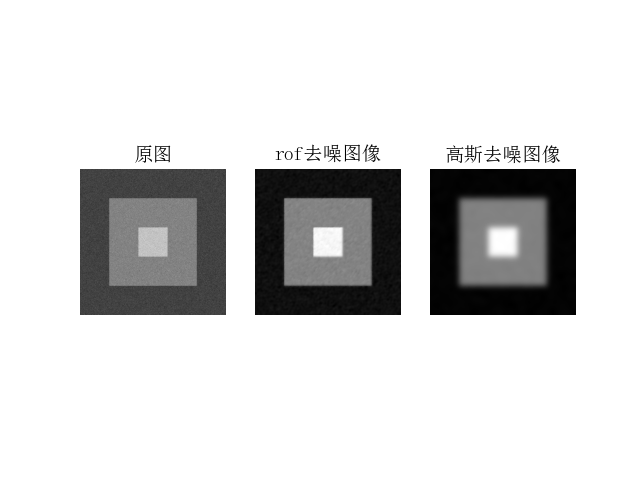
\includegraphics[width=0.8\textwidth]{Images/合成评估.png}
    \vspace{-7em}
    \caption{合成评估}
    \label{fig:synthesis_evaluation}
\end{figure}
我们可以看出原始图像显示为较暗的灰色正方形,ROF去噪图像则显示为白色正方形,通过Rudin-Osher-Fatemi模型处理后,图像变得更加明亮和清晰,有效减少噪声同时保留重要特征。高斯去噪图像也显示为白色正方形,通过高斯函数减少高频噪声,图像更加平滑。

之后我们对实际图像进行相同的处理。
\begin{figure}[ht]
    \centering
    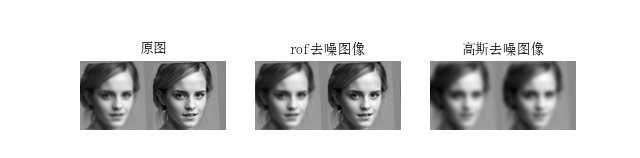
\includegraphics[width=1\textwidth]{Images/real.png}
    \vspace{-2em}
    \caption{实例评估}
    \label{fig:synthesis_evaluation}
\end{figure}
\FloatBarrier

从图像中我们可以看出,ROF模型可以保留原图像大趋势部分,使图像变得更加明亮和清晰,而高斯去噪将图像更加平滑,但也导致了图像变得更加模糊,从而导致不好的效果。

从上述比较可以看出,相较于高斯滤波,ROF模型具有更高的收敛性、稳定性。实际上,ROF模型解的存在是唯一的,这为模型的稳定性和可靠性提供了理论保障。\cite{rudin1994total}ROF模型不仅适用于去除高斯噪声和泊松噪声,还可以应用于其他类型的图像去噪任务中,具有广泛的应用前景。

\section{LLT模型}
同样,对比TV模型、LLT模型和改进的LLT模型的图像恢复效果.采用256×256像素的“Lena”图像
作为测试图像,如图3所示
\begin{figure}[ht]
    \centering
    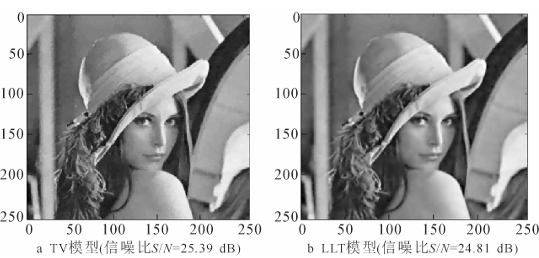
\includegraphics[width=0.5\textwidth]{Images/lena.png}
    \vspace{-1em}
    \caption{lena\cite{JSDN201705008}}
    \label{fig:synthesis_evaluation}
\end{figure}
\FloatBarrier
可以看出,LLT模型对图像光滑部分的恢复效果很好,但是在一定程度上模糊了图像的边缘。
    \cleardoublepage
    \titleformat{\chapter}[hang]{\linespread{1}\heiti\sanhao\bfseries\filright}{\thechapter}{1em}{}{}
\chapter{结论}
本文聚焦于计算机视觉领域中偏微分方程(PDE)在图像处理中的应用,特别是通过对比分析ROF全变分模型与LLT模型,探讨了不同模型在去噪任务中的特点与优劣。本文首先介绍了传统PDE去噪模型,为读者建立了对图像去噪的基本认识。随后,详细阐述了ROF全变分模型和LLT模型的原理、算法实现。

通过对ROF全变分模型的研究,我们发现该模型能够有效地去除图像中的噪声,同时保留图像的边缘信息。然而,ROF模型也存在一些局限性,如对于不同类型的噪声可能表现不佳,并且在处理过程中可能会产生伪影。相比之下,LLT模型作为一种基于二阶滤波器的概念,引入了递归平滑的思想,能够在保留图像细节的同时减少噪声的影响。LLT模型通过递归计算当前像素点的LLT值,并利用前一帧的LLT值来更新当前像素点的值,从而逐步提高图像质量。

本文还独立地利用编程技术直观展现了ROF全变分模型与LLT模型的差异。通过编写代码实现两种模型,并对同一组图像进行处理,我们观察到了它们在去噪效果上的显著差异。实验结果表明,LLT模型在某些情况下能够更好地保留图像的细节信息,而ROF模型则可能在边缘处产生模糊效应。

展望未来,PDE方程在图像处理领域的发展仍然充满潜力。随着深度学习等新技术的不断涌现,结合PDE的传统优势和新方法的创新思路,有望进一步提高图像处理的效果和效率。未来的研究可以探索如何将PDE与其他先进的图像处理技术相结合,以解决更复杂的图像处理问题,如超分辨率重建、图像分割等。此外,还可以考虑将PDE应用于其他相关领域,如医学影像分析、遥感图像处理等,以拓展其应用范围和影响力。
    \cleardoublepage
    \renewcommand{\thechapter}{}
    \bibliographystyle{Pages/sections/gbt7714-2005}
\bibliography{Pages/sections/bibliography}
\addcontentsline{toc}{chapter}{\bibname}
    % \cleardoublepage

    \include{data/acknowledgment}
    % \cleardoublepage
    \include{data/appendix}
  }

\end{document}
